%% notes-tex/multimodal/043-training-design/043-training-design.tex
%% [[experiments.043-expression-proteome-morphology]]
%% https://github.com/Mjvolk3/torchcell/tree/main/notes-tex/multimodal/043-training-design/043-training-design.tex
%%
%% Design review of the 043 training setup: notation (the Nature Biotechnology manuscript's,
%% extended where 043 needs more), the data and model flow, the model and the objective step
%% by step, the evaluation and decision rule, what the overnight round of 2026-10-22 measured,
%% and the open design questions. Dataset detail lives in the 043 datasets primer
%% (notes-tex/multimodal/043-datasets-primer/) and is not repeated.
%%
%% Build:  make            -> 043-training-design.pdf
%%         make check      -> gate
%%         make tables     -> rerun training_design_043_tables.py
%%         make diagrams   -> copy the rendered mermaid diagram into figures/
%%         make publish    -> upload the build to Zotero
%%
%% Ground truth: experiments/043-expression-proteome-morphology/scripts/train_043.py,
%% torchcell/models/cell_model_043.py, torchcell/models/readout_heads_043.py,
%% torchcell/losses/hl_gauss.py, torchcell/data/representation_043.py,
%% experiments/043-expression-proteome-morphology/scripts/global_split_043.py and the conf/
%% tree, at commit bed26f949.

\documentclass[10pt,a4paper]{article}
\usepackage[draft]{tcdoc}
\usepackage{float}
\usepackage{amsmath}
\usepackage{amssymb}

\emergencystretch=3.5em
\pdfstringdefDisableCommands{\def\secstatus#1{}}

%% GENERATED by experiments/043-expression-proteome-morphology/scripts/training_design_043_tables.py
%% SOURCE: results/overnight_2026_10_22_window_means.json, results/linear_evals_043.json, train_043_prep/prep_v1_routeA/meta.json (job 6134), conf/train_043_default.yaml. Do not edit by hand.
\newcommand{\tdTransferRecords}{$-$0.032}
\newcommand{\tdTransferBalanced}{$+$0.009}
\newcommand{\tdTransferPinball}{$-$0.020}
\newcommand{\tdNTrain}{50{,}767}
\newcommand{\tdNVaishnavTrain}{42{,}694}
\newcommand{\tdVaishnavPct}{84.1}
\newcommand{\tdGeneRecordsPerBatch}{1.27}
\newcommand{\tdVaishnavWeightEqual}{0.573}
\newcommand{\tdVaishnavWeightRecords}{0.841}
\newcommand{\tdKemmerenWeightEqual}{0.066}
\newcommand{\tdKemmerenPresent}{0.174}
\newcommand{\tdBalancedWeight}{0.111}
\newcommand{\tdStepsPerEpochJoint}{6{,}346}
\newcommand{\tdStepsPerEpochKemmeren}{151}


\title{\vspace{-1.5em}The 043 Training Setup\\
  {\large A design review: one model over expression, protein, isolate, segregant and
  promoter readouts, its objective, and how a transfer gain is decided}}
\author{Michael Volk}
\date{\today}

\begin{document}
\maketitle
\thispagestyle{empty}

%% notes-tex/multimodal/043-training-design/sections/0-abstract.tex
%% SOURCE: numbers from tables/macros.tex (training_design_043_tables.py) and
%% results/overnight_2026_10_22_window_means.json

\begin{abstract}
\noindent
Experiment 043 trains one model over nine datasets of the 043 store: deletion
transcriptomes and proteomes, natural-isolate transcriptomes and proteomes, segregant
single-cell expression, and a promoter library read by sort-seq. Every gene enters as a
composite of four frozen sequence embeddings plus a position term, a trunk encodes each
distinct reference context once, a perturbation operator applies the record's marks by
cross-attention, and two heads read a gene-level and a record-level value, with the dataset
entering only at the heads. The objective is a binned regression (HL-Gauss) on per-dataset
standardized targets, averaged within each dataset and weighted across datasets. Written
in the notation of the Nature Biotechnology manuscript, the setup is given equation by
equation, followed by the evaluation protocol and the rule that decides whether joint
training transfers to a dataset, the single-seed overnight runs of 2026-10-22 against the
linear bars, and the design questions left open. Under the uniform record sampler the
promoter library holds \tdVaishnavPct\% of the training records and carries an expected
\tdVaishnavWeightEqual{} of the batch objective's weight; the step-matched transfer on
Kemmeren 2014 read \tdTransferRecords{}, \tdTransferBalanced{} and \tdTransferPinball{}
for the three complete joint runs, one seed each and below the decision rule.
\end{abstract}


\vspace{0.5em}
\tccontents
\clearpage

%% notes-tex/multimodal/043-training-design/sections/1-notation.tex
%% SOURCE: hand-authored notation contract. Paper rows copy paper/nature-biotech/sections/methods.tex
%% (Table tab:notation and Eqs. objective to loss); 043 rows name the code symbol they stand for
%% (torchcell/models/cell_model_043.py, torchcell/losses/hl_gauss.py, train_043.py).

\section{Notation\secstatus{todo}}
\label{sec:notation}

The symbols are the manuscript's (Methods, Table ``Notation'', and Eqs.\ for the encoder,
the perturbation operator, the readouts and the loss), reused with the same meaning.
Where 043 needs more, the symbol is defined once in the second block of
Table~\ref{tab:notation} and marked ``043''. Four manuscript symbols carry a narrower
meaning here and say so in their rows: the task index becomes the dataset index $s$,
the perturbation tokens are the record's marks, the type $\tau_t$ is a change type, and the
mask $m$ marks measured entries only, since 043 marks carry no magnitude. Two manuscript
symbols whose objects 043 does not build are reused: $s$, the gene-set index of the
morphology head, and $\lambda$, the graph-prior weights, absent because 043 masks attention
instead of regularizing it. Within each block the rows are alphabetical by the symbol's
letter name.

\begingroup
\footnotesize
\setlength{\tabcolsep}{4pt}
\begin{longtable}{>{\raggedright\arraybackslash}p{34mm}>{\raggedright\arraybackslash}p{128mm}>{\raggedright\arraybackslash}p{10mm}}
\caption[]{\textbf{Notation.} First block: manuscript symbols as 043 uses them. Second
block: symbols 043 adds. Shapes are per record unless a batch dimension is written.
Numbers are the values of the overnight runs of 2026-10-22
(\file{conf/train_043_default.yaml} with \texttt{data.batch\_size=8}).}\label{tab:notation}\\
\toprule
Symbol & Meaning in 043 & Source \\
\midrule
\endfirsthead
\toprule
Symbol & Meaning in 043 & Source \\
\midrule
\endhead
$a,\ h$ & attention head index, number of heads; $h = 9$ in the trunk and the operator & paper \\
$A^{(k)}$ & relation-$k$ adjacency over genes; nine relations, one per head of the masked trunk layer, used as a hard mask (Eq.~\ref{eq:mask}), not as a KL prior & paper \\
$\alpha^{(\ell,a)}$ & trunk self-attention map of layer $\ell$, head $a$ & paper \\
$B$ & records per batch; 8 in every overnight run (the config default is 16) & paper \\
$\beta^{a}_{i,t}$ & operator cross-attention weight of query $i$ on mark $t$ in head $a$; the softmax also runs over the null key $\varnothing$ & paper \\
$d,\ d_k$ & model width $d = 144$; head width $d_k = d/h = 16$ & paper \\
$\operatorname{Embed},\ \mathbf{E}$ & entity encoder; learned lookup table. Every learned lookup of 043 is an $\mathbf{E}$ with a superscript naming it: $\mathbf{E}^{\mathrm{gap}}$, $\mathbf{E}^{\mathrm{chr}}$, $\mathbf{E}^{\mathrm{pgap}}$, $\mathbf{E}^{\mathrm{par}}$, $\mathbf{E}^{\mathrm{type}}$, $\mathbf{E}^{\mathrm{data}}$, $\mathbf{E}^{\mathrm{env}}$ & paper \\
$\varepsilon$ & environment; enters only through the token $\mathbf{c}^{\mathrm{env}}$ at the heads & paper \\
$F_\theta$ & trunk (encoder), $H_c = F_\theta(G_c)$ & paper \\
$\operatorname{FFN},\ \operatorname{LN},\ \operatorname{MLP}$ & position-wise feed-forward network, layer normalization, two-layer perceptron (Linear, GELU, dropout 0.1, Linear) & paper \\
$G,\ g_i,\ N$ & reference cell; gene $i$ of the shared index; $N = 6{,}607$ & paper \\
$H,\ h_i,\ h_{\mathrm{CLS}}$ & trunk states $(h_{\mathrm{CLS}}, h_1, \ldots, h_N) \in \mathbb{R}^{(N+1)\times d}$; $H^{(\ell)}$ after layer $\ell$ & paper \\
$H_{\mathrm{pert}},\ h^{\mathrm{pert}}_i$ & operator output, same shape as $H$ & paper \\
$\ell,\ L$ & trunk layer index, number of layers; $L = 4$ & paper \\
$\mathcal{L},\ \mathcal{L}_y$ & loss; supervised objective of a batch (Eq.~\ref{eq:objective}). 043 has no graph term, so $\mathcal{L} = \mathcal{L}_y$ & paper \\
$m_{b,i}$ & 1 when entry $i$ of record $b$ is measured, else 0 (the manuscript's $m_t^{(b)}$) & paper \\
$M_b$ & number of marks of record $b$ (the manuscript's $M$) & paper \\
$p,\ \mathbf{p}_t,\ \mathbf{P}$ & perturbation set; its tokens are the record's marks $t = 1, \ldots, M_b$ (Eq.~\ref{eq:markkey}) & paper \\
$\mathcal{R}_\phi$ & decoder: the gene head and the record head (Eqs.~\ref{eq:genehead},~\ref{eq:rechead}) & paper \\
$\mathcal{T}_\psi$ & perturbation operator (Eqs.~\ref{eq:opattn},~\ref{eq:rezero}) & paper \\
$\tau_t,\ \mathbf{t}_{\tau}$ & type of mark $t$, here a change type $\tau_t \in \mathcal{C}$; its learned embedding & paper \\
$\Theta$ & all trainable parameters, 1.85\,M in the overnight runs (job 6136 log) & paper \\
$W_Q, W_K, W_V, W_O$ & query, key, value and output maps & paper \\
$w_s$ & weight of dataset $s$ in the objective (the manuscript's task weight $w_t$) & paper \\
$x_i,\ x_{\mathrm{CLS}}$ & input token of gene $i$ (Eq.~\ref{eq:token}); learned CLS token & paper \\
$y,\ \hat y$ & released label, prediction & paper \\
\midrule
$\bar{\mathbf{k}}_b$ & mean of the mark keys of record $b$ (the primer's $z_S$, renamed because $z$ is the target here); zero without marks & 043 \\
$\mathbf{b}^{\mathrm{gene}}_s,\ \mathbf{b}^{\mathrm{rec}}_s$ & learned per-dataset bias of the gene and the record head, $\in \mathbb{R}^{n_{\mathrm{out}}}$ & 043 \\
$\mathcal{B},\ n_s(\mathcal{B}),\ \mathcal{S}_{\mathcal{B}}$ & a batch of records; the records of dataset $s$ in it; the datasets with a measured entry in it & 043 \\
$c,\ G_c,\ H_c$ & reference context (S288C, or an isolate under route A); its cell; its trunk states & 043 \\
$\mathbf{c}_b$ & conditioning token $[\mathbf{c}^{\mathrm{type}}; \mathbf{c}^{\mathrm{data}}; \mathbf{c}^{\mathrm{env}}] \in \mathbb{R}^{40}$ of record $b$ (Eq.~\ref{eq:cond}) & 043 \\
$\mathcal{C}$ & change-type vocabulary: reference, deletion, variant, loss of function, absent, present, promoter & 043 \\
$\chi$ & node of the experiment-type path (Eq.~\ref{eq:typetoken}) & 043 \\
$\Delta$ & HL-Gauss bin width, $8/32 = 0.25$ in $z$ & 043 \\
$\eta_{s,i},\ \mu_s,\ \sigma_s$ & per-gene center (zero unless the dataset is centered per gene), pooled mean and standard deviation of dataset $s$ over its training rows & 043 \\
$\operatorname{Four}(\xi)$ & Fourier features $[\sin(2\pi 2^f \xi), \cos(2\pi 2^f \xi)]_{f=0}^{7} \in \mathbb{R}^{16}$ & 043 \\
$\gamma_u$ & quantile level $u/20$, $u = 1, \ldots, 19$ & 043 \\
$\kappa,\ \mathcal{K}$ & typed-gap kind of a block slot; the 12 kinds of \texttt{GapKind} (no allele, locus gap, short flank, \ldots, ambiguous sequence) & 043 \\
$\mathbf{k}_{\varnothing}$ & learned null key of the operator, one per head, with value zero & 043 \\
$\lambda_0, \lambda_1, \lambda_2$ & coefficients of the fitted doubles rung (Eq.~\ref{eq:fitted}) & 043 \\
$n_{\mathrm{bin}},\ n_q,\ n_{\mathrm{out}}$ & HL-Gauss bins (32); pinball quantiles (19); head output width ($n_{\mathrm{bin}}$, $n_q$ or 1) & 043 \\
$n_s,\ n$ & training records of dataset $s$; $n = \sum_s n_s = \tdNTrain$ & 043 \\
$n_{\mathrm{ep}},\ n_{\mathrm{step}}$ & epochs and optimizer steps of a run & 043 \\
$\nu^{\mathrm{chr}}_{c,i},\ \nu^{\mathrm{gene}}_{c,i}$ & copy number of gene $i$'s chromosome relative to the basal ploidy, and of the gene, in context $c$ & 043 \\
$o_t$ & allele parent of mark $t$ (segregants; row 0 is ``no parent'') & 043 \\
$\hat{\mathbf{o}}_{b,i}$ & head output for entry $i$ of record $b$, $\in \mathbb{R}^{n_{\mathrm{out}}}$ & 043 \\
$\omega_u(z),\ \hat\omega_u$ & target and predicted mass of HL-Gauss bin $u$ & 043 \\
$q,\ \mathcal{Q}$ & frozen block index, $\mathcal{Q} = \{\mathrm{up}, \mathrm{down}, \mathrm{prot}, \mathrm{calm}\}$ & 043 \\
$s,\ \mathcal{S},\ s(b)$ & dataset index; the training datasets of an arm ($|\mathcal{S}| = 9$ for \texttt{joint\_9}); the dataset of record $b$ & 043 \\
$\operatorname{stat}_e$ & an evaluation statistic at epoch $e$; $\overline{\operatorname{stat}}$ its registered-window mean & 043 \\
$\operatorname{tr}_s$ & pre-standardization transform of dataset $s$ & 043 \\
$u$ & output component index (bin or quantile) & 043 \\
$\upsilon_u,\ \bar\upsilon_u$ & HL-Gauss bin edges and centers & 043 \\
$\mathcal{W}$ & registered window: the epochs whose evaluations are averaged & 043 \\
$x^{(q)}_{c,i},\ d_q$ & frozen vector of block $q$ for gene $i$ in context $c$; its width, $(768, 768, 1024, 768)$ & 043 \\
$\xi_i$ & relative midpoint of gene $i$ on its chromosome, in $[0,1]$ & 043 \\
$z_{b,i},\ \hat z_{b,i}$ & standardized target (Eq.~\ref{eq:standardize}); point prediction in $z$ & 043 \\
$\zeta_{\mathrm{attn}},\ \zeta_{\mathrm{ffn}}$ & ReZero gates of the operator, initialized at zero & 043 \\
\bottomrule
\end{longtable}
\endgroup

%% notes-tex/multimodal/043-training-design/sections/2-flow.tex
%% SOURCE: the diagram's numbers and their files are listed in its Dendron note,
%% notes/experiments.043-expression-proteome-morphology.mermaid.training-design.md

\section{Data and model flow\secstatus{todo}}
\label{sec:flow}

Figure~\ref{fig:flow} follows a record from the raw store to the number the decision rule
reads. The store and its datasets are described in the 043 datasets primer
(\file{notes-tex/multimodal/043-datasets-primer/}, Secs.\ 1 to 4 and 6); what follows starts
where the primer stops, at the representation the trainer consumes. Two facts set the
shape of the pipeline. First, the representation holds keys, not vectors: each gene slot
of a reference context carries one key per frozen block, or a typed gap, and the trainer
reads the vectors of exactly the keys its records use, failing on a missing one.
Second, the reference context is part of the input: a deletion, segregant or promoter
record is read on S288C, an isolate on its own alleles (route A), so a batch carries
between one and $B$ distinct contexts, and the trunk runs once per distinct context.

%% SOURCE: notes/experiments.043-expression-proteome-morphology.mermaid.training-design.md, rendered by
%% notes/assets/publish/scripts/mermaid_pdf.sh, copied and scaled to 180 mm by `make diagrams`
\begin{figure}[htbp]\centering
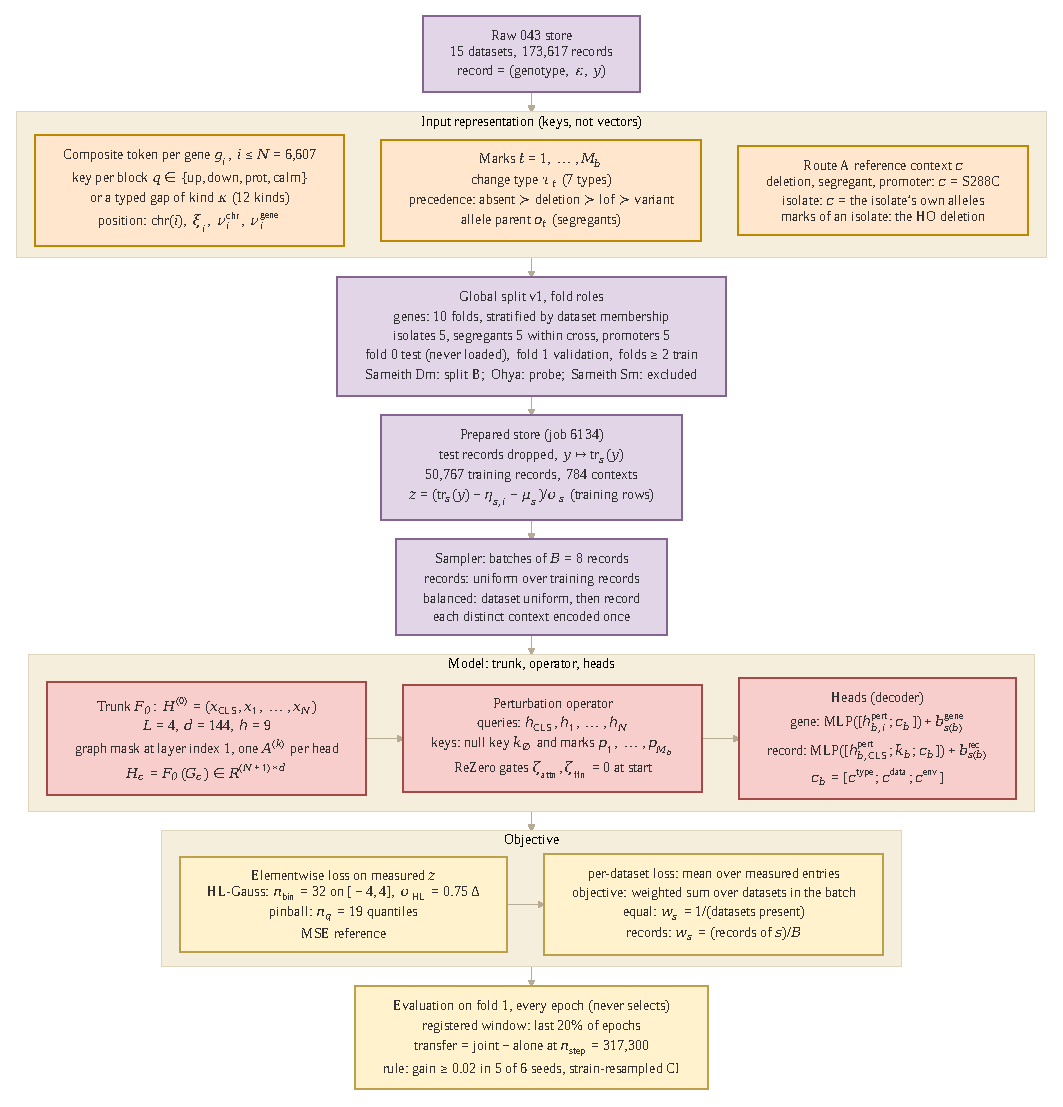
\includegraphics[width=\textwidth]{figures/mermaid-training-design.pdf}\par\vspace{2pt}
\caption[]{\textbf{The 043 training pipeline, from the raw store to the
registered-window read.} Purple, data: the store, the fold roles of the global split, the
prepared store (job 6134; test records dropped before any label is loaded) and the batch.
Orange, input side: the composite token per gene with its position features, the marks
with their change types and allele parents, and the route-A reference context. Red,
model: trunk, perturbation operator and heads. Yellow, objective and evaluation. The 784
contexts of the prepared store are S288C and the 783 isolates outside fold 0. In the
rendered math, vectors written bold in the text ($\mathbf{c}_b$, $\mathbf{p}_t$,
$\bar{\mathbf{k}}_b$) appear in the regular face. Rendered 212 mm wide and placed at
180 mm, a scale of 0.85.}
\label{fig:flow}
\end{figure}
%% Generated by notes/assets/publish/scripts/mermaid_pdf.sh from
%% notes/experiments.043-expression-proteome-morphology.mermaid.training-design.md

\notesec{Stages}
The global split assigns every record one role before anything trains
(Sec.~\ref{sec:split}). The prepare stage (\file{train_043.py} \texttt{-{}-stage prepare}, job 6134)
reads every record of the arm's datasets with its route-A representation, drops the test
records, applies the per-dataset transform $\operatorname{tr}_s$ and writes keys, marks,
contexts, targets and the nine gene--gene edge lists into one store. Training fits the
standardization on the training rows, builds the model, and logs the training objective
every 50 steps and the validation pass every evaluation epoch. Nothing downstream of the
prepared store reads fold 0.

%% notes-tex/multimodal/043-training-design/sections/3-model.tex
%% SOURCE: torchcell/models/cell_model_043.py (CompositeToken, PositionTerm, CellTrunk043,
%% MarkOperator043, CellModel043), torchcell/models/readout_heads_043.py,
%% torchcell/models/genotype_tokens_043.py (ChangeType, CHANGE_PRECEDENCE),
%% torchcell/models/equivariant_cell_graph_transformer.py (GraphRegularizedTransformerLayer),
%% torchcell/data/representation_043.py (GapKind, PositionGap), train_043.py (EXP_TYPE_PATHS,
%% build_model), conf/train_043_default.yaml; parameter count and table rows from the
%% job 6136 log.

\section{Model, step by step\secstatus{todo}}
\label{sec:model}

The model keeps the manuscript's factorization $\hat f_\theta = \mathcal{R}_\phi \circ
\mathcal{T}_\psi \circ F_\theta$ (Methods, ``Problem setup'') and changes what enters it:
the input token of a gene is a function of the reference context, the perturbation tokens
are typed marks, and the decoder is two shared heads with the dataset entering only at
their input and output. Shapes are given for one record unless a batch axis is written;
$C$ is the number of distinct contexts in a batch.

\subsection{The gene token\secstatus{todo}}
\label{sec:token}

\notesec{Step 1, the four frozen blocks}
For context $c$ and gene $i$, each block $q \in \mathcal{Q}$ holds either a key or a typed
gap $\kappa \in \mathcal{K}$. A key indexes a frozen fp16 vector $x^{(q)}_{c,i} \in
\mathbb{R}^{d_q}$: the FUDT upstream encoder on the 1{,}003 bp window ($d_{\mathrm{up}} =
768$), the FUDT downstream encoder on the 300 bp window ($d_{\mathrm{down}} = 768$),
ProtT5-XL on the protein ($d_{\mathrm{prot}} = 1024$) and CaLM on the coding sequence
($d_{\mathrm{calm}} = 768$). Each block is normalized and projected separately,
\begin{equation}
\tilde x^{(q)}_{c,i} =
\begin{cases}
W^{(q)} \operatorname{LN}^{(q)}\!\big(x^{(q)}_{c,i}\big) + b^{(q)} & \text{if block } q \text{ of gene } i \text{ has a key in } c,\\[2pt]
\mathbf{E}^{\mathrm{gap}}_{q,\kappa} & \text{if it carries the gap } \kappa,
\end{cases}
\qquad W^{(q)} \in \mathbb{R}^{d \times d_q},
\label{eq:block}
\end{equation}
so a gap is a learned vector of its own kind and block and is never filled with another
sequence's vector. The vectors stay frozen; $\operatorname{LN}^{(q)}$, $W^{(q)}$, $b^{(q)}$
and $\mathbf{E}^{\mathrm{gap}} \in \mathbb{R}^{(4 \cdot 12) \times d}$ train. The overnight
runs held 929{,}348, 326{,}255, 329{,}430 and 514{,}189 rows of the four tables on the card,
3.39 GB (job 6136 log).

\notesec{Step 2, the composite}
The four projections are summed,
\begin{equation}
\tilde x_{c,i} = \sum_{q \in \mathcal{Q}} \tilde x^{(q)}_{c,i} \in \mathbb{R}^{d}.
\label{eq:composite}
\end{equation}

\notesec{Step 3, the position term}
Gene $i$ lies on chromosome $\operatorname{chr}(i) \in \{0, \ldots, 16\}$ (0 is the
mitochondrion) at relative midpoint $\xi_i \in [0,1]$ of the reference. With $\nu^{\mathrm{chr}}_{c,i}$
the copy number of that chromosome relative to the basal ploidy (1 except on aneuploid
isolate chromosomes) and $\nu^{\mathrm{gene}}_{c,i}$ the gene's copy number,
\begin{equation}
\operatorname{pos}_{c,i} =
\nu^{\mathrm{chr}}_{c,i}\, \mathbf{E}^{\mathrm{chr}}_{\operatorname{chr}(i)}
+ W_{\xi} \operatorname{Four}(\xi_i) + b_{\xi}
+ \mathbf{w}_{\nu}\big(\log_2(\nu^{\mathrm{gene}}_{c,i} + 1) - 1\big) + \mathbf{b}_{\nu}
+ \mathbf{E}^{\mathrm{pgap}}_{\kappa'_{c,i}},
\label{eq:pos}
\end{equation}
with $\mathbf{E}^{\mathrm{chr}} \in \mathbb{R}^{19 \times d}$ (17 chromosomes and two rows for
off-graph tokens, an accessory ORF and the reporter construct), $W_{\xi} \in \mathbb{R}^{d
\times 16}$ and $\mathbf{w}_\nu, \mathbf{b}_\nu \in \mathbb{R}^{d}$. The copy feature is 0 at
one copy and $-1$ at zero copies. An unknown copy number (a ploidy the source did not report,
a value the pangenome matrix does not release) drops its term and selects the learned
position-gap row $\kappa'_{c,i}$ of $\mathbf{E}^{\mathrm{pgap}} \in \mathbb{R}^{4 \times d}$
(row 0 when nothing is unknown).

\notesec{Step 4, the input token}
The manuscript's node feature $x_i = \operatorname{Embed}(g_i)$ becomes context dependent,
\begin{equation}
x_{c,i} = \tilde x_{c,i} + \operatorname{pos}_{c,i},
\qquad
H^{(0)}_c = (x_{\mathrm{CLS}}, x_{c,1}, \ldots, x_{c,N}) \in \mathbb{R}^{(N+1) \times d}.
\label{eq:token}
\end{equation}
For S288C every slot has its reference keys; under route A an isolate's slots carry the
isolate's own alleles, with the genes outside the released allele set and the genes the
record calls absent as gaps.

\subsection{The trunk\secstatus{todo}}
\label{sec:trunk}

\notesec{Step 5, the layers}
$F_\theta$ is four layers of width $d = 144$ with $h = 9$ heads of width $d_k = 16$. The
layer is the manuscript's Eqs.\ for the queries, keys, values and attention map, but
post-normalized, where the manuscript writes the pre-normalized form,
\begin{equation}
\hat H^{(\ell)} = \operatorname{LN}\!\Big(H^{(\ell-1)} + \operatorname{Drop}\big(\big[O^{(\ell,1)} \Vert \cdots \Vert O^{(\ell,h)}\big] W_O^{(\ell)}\big)\Big),
\qquad
H^{(\ell)} = \operatorname{LN}\!\Big(\hat H^{(\ell)} + \operatorname{Drop}\big(\operatorname{FFN}^{(\ell)}(\hat H^{(\ell)})\big)\Big).
\label{eq:layer}
\end{equation}

\notesec{Step 6, the graph mask}
In layer $\ell = 2$ (\texttt{mask\_layers: [1]}, counted from zero) head $a$ may attend only
along graph $k(a)$; the other three layers are unmasked. With $A^{(k)}$ symmetrized,
\begin{equation}
\alpha^{(2,a)} = \operatorname{softmax}\!\Big(\frac{Q^{(2,a)} (K^{(2,a)})^{\top}}{\sqrt{d_k}} + \Gamma^{(a)}\Big),
\qquad
\Gamma^{(a)}_{ij} =
\begin{cases}
0 & \text{if } A^{(k(a))}_{ij} = 1,\ A^{(k(a))}_{ji} = 1,\ i = j, \text{ or } i \text{ or } j \text{ is the CLS},\\
-\infty & \text{otherwise},
\end{cases}
\label{eq:mask}
\end{equation}
with $k(0), \ldots, k(8)$ the physical, regulatory and TFLink graphs and the STRING 12.0
neighborhood, fusion, co-occurrence, coexpression, experimental and database channels.
The objective carries no $\Omega_k$ term: 043 takes the manuscript's $\lambda \to \infty$
limit of graph-regularized attention at one layer and leaves the rest free.

\notesec{Step 7, one encode per context}
Each distinct context of a batch is encoded once, $H_c = F_\theta(G_c) \in \mathbb{R}^{(N+1)
\times d}$, a $[C, N+1, d]$ tensor, and record $b$ reads $H_{c(b)}$. The trunk trains, so
nothing is cached across batches.

\subsection{Marks and the perturbation operator\secstatus{todo}}
\label{sec:operator}

\notesec{Step 8, change types}
Each gene of a genotype has one change type in $\mathcal{C}$. When the source gives a gene
several, the first in the order absent, deletion, loss of function, variant, present,
promoter wins: a gene that is gone outranks a call on its sequence, which outranks a
variant that is still expressed. A mark is a token the operator attends to: a deleted gene,
a gene a segregant inherits from a non-BY parent (a variant, with that parent as $o_t$), the
HO deletion of an isolate under route A, an isolate's present accessory ORF (off-graph), and
Vaishnav's reporter, an off-graph token whose upstream key is the variant's 1{,}003 bp
construct window. Under route A the isolate's variants live in its context, not in its
marks. The overnight runs kept at most 1{,}024 marks per record (\texttt{data.mark\_cap}:
absent, deletion and loss-of-function marks first, then a fixed per-record random subset),
a smoke-time truncation the design does not have; N'Guessan 2025 records carry a median of
2{,}910 marks (job 6120).

\notesec{Step 9, the mark key}
Mark $t$ of record $b$ has the composite and position of its gene in the record's context
(or of its off-graph token, with the replicon row of $\mathbf{E}^{\mathrm{chr}}$ and the
Fourier term zeroed), plus its change type and allele parent,
\begin{equation}
\tilde{\mathbf{p}}_t = \tilde x_{t} + \operatorname{pos}_{t} + \mathbf{t}_{\tau_t} + \mathbf{E}^{\mathrm{par}}_{o_t},
\qquad
\mathbf{p}_t = W_p \operatorname{LN}(\tilde{\mathbf{p}}_t) + b_p + \mathbf{1}[\text{mark } t \text{ is on the graph}]\; h_{c(b),\,j_t},
\label{eq:markkey}
\end{equation}
where $j_t$ is the marked gene and $\mathbf{E}^{\mathrm{par}}_0 = 0$ is ``no parent''. This is
the manuscript's token $\mathbf{p}_t = r(e_t) + \mathbf{t}_{\tau_t} + m_t \mathbf{w}$ with two
changes: the projected mark token is added for in-cell genes as well, and there is no
magnitude term. $\mathbf{P}_b \in \mathbb{R}^{M_b \times d}$, padded to $[B, \max_b M_b, d]$.

\notesec{Step 10, cross-attention with a null sink}
Every token of the context, the CLS included, is a query. Each head adds a learned null key
$\mathbf{k}_{\varnothing}$ with value zero, so a record without marks attends only to it and a
record with one mark does not see a degenerate softmax,
\begin{equation}
\beta^{a}_{i,t} = \operatorname*{softmax}_{t \in \{\varnothing, 1, \ldots, M_b\}} \frac{(h_i W^{a}_Q) \cdot \mathbf{k}^{a}_t}{\sqrt{d_k}},
\quad
\mathbf{k}^{a}_t = \mathbf{p}_t W^{a}_K,
\quad
\Delta h_i = \Big[\textstyle\sum_{t \ge 1} \beta^{1}_{i,t}\, \mathbf{p}_t W^{1}_V \,\Big\Vert \cdots \Big\Vert\, \sum_{t \ge 1} \beta^{h}_{i,t}\, \mathbf{p}_t W^{h}_V\Big] W_O,
\label{eq:opattn}
\end{equation}
for $i \in \{\mathrm{CLS}, 1, \ldots, N\}$; the null term contributes weight but no value.

\notesec{Step 11, the ReZero residual}
Where the manuscript's operator normalizes, 043 gates,
\begin{equation}
h'_i = h_i + \zeta_{\mathrm{attn}} \operatorname{Drop}(\Delta h_i),
\qquad
h^{\mathrm{pert}}_i = h'_i + \zeta_{\mathrm{ffn}} \operatorname{Drop}\big(\operatorname{FFN}(h'_i)\big),
\qquad
H_{\mathrm{pert}} = \mathcal{T}_\psi(H_{c(b)}, p_b) \in \mathbb{R}^{(N+1) \times d},
\label{eq:rezero}
\end{equation}
with $\zeta_{\mathrm{attn}} = \zeta_{\mathrm{ffn}} = 0$ at initialization, so at step 0 the
operator is the identity and $H_{\mathrm{pert}} = H_{c(b)}$. The record-level summary of the
marks is
\begin{equation}
\bar{\mathbf{k}}_b = \frac{1}{\max(M_b, 1)} \sum_{t=1}^{M_b} \mathbf{p}_t \in \mathbb{R}^{d}.
\label{eq:summary}
\end{equation}

\subsection{Conditioning tokens and heads\secstatus{todo}}
\label{sec:heads}

\notesec{Step 12, the experiment-type token}
Each dataset reads one phenotype class of the schema, and the class enters as the sum of
one learned row per node of its path,
\begin{equation}
\mathbf{c}^{\mathrm{type}}_b = \sum_{\chi \in \operatorname{path}(\operatorname{class}(s(b)))} \mathbf{E}^{\mathrm{type}}_{\chi} \in \mathbb{R}^{16},
\label{eq:typetoken}
\end{equation}
where a path runs root, group, leaf: phenotype, expression, then the microarray (Kemmeren),
RNA-seq (Caudal) or single-cell (Boocock, N'Guessan) class; phenotype, protein, then protein
abundance (Messner, Zelezniak, Muenzner) or turnover (Muenzner turnover); phenotype,
promoter, pooled sort-seq (Vaishnav). The path is the minimal differential subset of the
ontology DAG for these six leaves: it keeps the one level that separates them into the three
readout groups the heads share, so two leaves under one group share that group's row and
differ by their own. The group nodes are modeling-side groups, not schema classes
(\file{train_043.py}, \texttt{EXP\_TYPE\_PATHS}); the root is on every path and acts as a
shared offset. The flat alternative, one row per leaf, is \texttt{exp\_type\_mode: flat}
(Sec.~\ref{sec:open}).

\notesec{Step 13, the conditioning token}
The dataset and the environment are flat lookups,
\begin{equation}
\mathbf{c}_b = \big[\mathbf{c}^{\mathrm{type}}_b ;\ \mathbf{E}^{\mathrm{data}}_{s(b)} ;\ \mathbf{E}^{\mathrm{env}}_{\varepsilon(b)}\big] \in \mathbb{R}^{16 + 8 + 16 = 40},
\label{eq:cond}
\end{equation}
over the nine datasets and nine environments of the prepared store.

\notesec{Step 14, the gene head}
Every gene-level dataset shares one head that reads the gene's own perturbed state, the
manuscript's equivariant readout with the conditioning token appended,
\begin{equation}
\hat{\mathbf{o}}_{b,i} = \operatorname{MLP}_{\mathrm{gene}}\big([h^{\mathrm{pert}}_{b,i} ;\ \mathbf{c}_b]\big) + \mathbf{b}^{\mathrm{gene}}_{s(b)} \in \mathbb{R}^{n_{\mathrm{out}}},
\qquad i = 1, \ldots, N,
\label{eq:genehead}
\end{equation}
with $\operatorname{MLP}_{\mathrm{gene}}: \mathbb{R}^{184} \to \mathbb{R}^{128} \to
\mathbb{R}^{n_{\mathrm{out}}}$, a $[B_{\mathrm{gene}}, N, n_{\mathrm{out}}]$ output.

\notesec{Step 15, the record head}
Vaishnav's one value per promoter is read from the perturbed CLS, the mark summary and the
conditioning token,
\begin{equation}
\hat{\mathbf{o}}_{b} = \operatorname{MLP}_{\mathrm{rec}}\big([h^{\mathrm{pert}}_{b,\mathrm{CLS}} ;\ \bar{\mathbf{k}}_b ;\ \mathbf{c}_b]\big) + \mathbf{b}^{\mathrm{rec}}_{s(b)} \in \mathbb{R}^{n_{\mathrm{out}}},
\label{eq:rechead}
\end{equation}
with $\operatorname{MLP}_{\mathrm{rec}}: \mathbb{R}^{328} \to \mathbb{R}^{128} \to
\mathbb{R}^{n_{\mathrm{out}}}$; it replaces the manuscript's perturbed-gene mean in the
interaction head by the mark-key mean of Eq.~\ref{eq:summary}.

\notesec{The per-dataset term is a bias}
The design calls for a per-dataset affine at the head, $a_s f(\cdot) + \mathbf{b}_s$.
\texttt{CellModel043} builds the gene head with \texttt{per\_dataset\_affine=False} and adds
$\mathbf{b}_s$ alone, so the scale $a_s$ is fixed at 1 in every run so far. Under HL-Gauss
$\mathbf{b}_s$ adds to the 32 logits, a learned prior histogram per dataset. The dataset
id therefore enters in two places, both at the heads: $\mathbf{E}^{\mathrm{data}}$ inside
$\mathbf{c}_b$ and the bias. It never reaches the trunk or the operator.

%% notes-tex/multimodal/043-training-design/sections/4-objective.tex
%% SOURCE: torchcell/losses/hl_gauss.py (HLGaussLoss, fit_standardization),
%% torchcell/losses/distributional.py (pinball), torchcell/models/cell_model_043.py
%% (ReadoutLoss043), train_043.py (SPECS, transform_target, loss_sums, combine_loss,
%% balanced_batches, batch_loader, predict, evaluate, OptimConfig), conf/loss/*.yaml,
%% conf/weighting/*.yaml; batch shares through tables/t2-batch-share-rows.tex and
%% tables/macros.tex (training_design_043_tables.py); standardization sha256 from the job 6136 log.

\section{Objective, step by step\secstatus{todo}}
\label{sec:objective}

\subsection{Targets\secstatus{todo}}
\label{sec:targets}

\notesec{Step 1, the transform}
Each dataset's released value is first put on a scale where differences are comparable,
$\tilde y_{b,i} = \operatorname{tr}_s(y_{b,i})$: as released for Kemmeren (already a
$\log_2$ ratio to wild type) and Vaishnav (a sort-seq level); the $\log_2$ ratio to the
reference for Messner; the difference to the reference for Zelezniak; $\log_2(y+1)$ of TPM
for Caudal; $\log_2 y$ of positive values for Muenzner protein and turnover; and
$\log_2(10^{6} y / \text{UMI total} + 1)$ for the Boocock and N'Guessan counts, where a
gene a record omits is a released zero. The primer's table of output scales gives the
reasons per dataset.

\notesec{Step 2, standardization per dataset}
On the training rows of dataset $s$ only,
\begin{equation}
z_{b,i} = \frac{\tilde y_{b,i} - \eta_{s,i} - \mu_s}{\sigma_s},
\qquad
m_{b,i} = \mathbf{1}\big[z_{b,i} \text{ is finite}\big],
\label{eq:standardize}
\end{equation}
where $\eta_{s,i}$ is the mean of gene $i$ over the training rows that measure it for the
five panel datasets centered per gene (Caudal, Muenzner protein and turnover, Boocock,
N'Guessan) and zero for the rest, and $\mu_s$, $\sigma_s$ are the mean and standard
deviation pooled over every centered training value of $s$. A gene with no training value
has no center, so its $z$ is missing rather than zero. The fitted statistics are one
pydantic record pinned by sha256 (\texttt{0d5df0f0\ldots} in the overnight runs, job 6136
log). Counts never detected in a Boocock or N'Guessan training row are not targets.

\subsection{Elementwise losses\secstatus{todo}}
\label{sec:elementwise}

\notesec{Step 3, HL-Gauss bins}
The main loss (decision O4 of the primer) bins $z$ into $n_{\mathrm{bin}} = 32$ bins on
$[-4, 4]$ of width $\Delta = 0.25$, with interior edges $\upsilon_u = -4 + u\Delta$ for $u =
1, \ldots, 31$, the outer edges opened to $\upsilon_0 = -\infty$ and $\upsilon_{32} =
+\infty$, and nominal centers $\bar\upsilon_u = -4 + (u - \tfrac12)\Delta$.

\notesec{Step 4, the Gaussian histogram target}
A measured $z$ becomes the mass a normal $\mathcal{N}(z, \sigma_{\mathrm{HL}}^2)$ puts in
each bin, with $\sigma_{\mathrm{HL}} = 0.75\Delta = 0.1875$ and $\Phi$ the standard normal
distribution function,
\begin{equation}
\omega_u(z) = \Phi\!\Big(\frac{\upsilon_u - z}{\sigma_{\mathrm{HL}}}\Big) - \Phi\!\Big(\frac{\upsilon_{u-1} - z}{\sigma_{\mathrm{HL}}}\Big),
\qquad u = 1, \ldots, n_{\mathrm{bin}},
\qquad \sum_{u} \omega_u(z) = 1.
\label{eq:hltarget}
\end{equation}
Because the edge bins are open, a target beyond $\pm 4$ still has a histogram that sums to
one; its mass sits in the edge bin.

\notesec{Step 5, the cross-entropy}
The head's $n_{\mathrm{out}} = 32$ outputs are logits,
\begin{equation}
\hat\omega_u = \frac{\exp(\hat o_u)}{\sum_{u'} \exp(\hat o_{u'})},
\qquad
\mathcal{L}^{\mathrm{HL}}(\hat{\mathbf{o}}, z) = -\sum_{u=1}^{n_{\mathrm{bin}}} \omega_u(z) \log \hat\omega_u.
\label{eq:hlce}
\end{equation}

\notesec{Step 6, the point prediction}
The prediction scored by every correlation is the expectation over the nominal centers,
\begin{equation}
\hat z = \sum_{u=1}^{n_{\mathrm{bin}}} \hat\omega_u\, \bar\upsilon_u \in [-3.875,\ 3.875],
\label{eq:hlpoint}
\end{equation}
a convex combination of the centers, so it lies inside the outermost centers and moves
toward the middle of the histogram when the predicted mass spreads. The trainer also logs
the entropy of $\hat\omega$ and the fraction of measured entries whose argmax bin is within
one bin of the target's.

\notesec{Step 7, the pinball arm}
The quantile arm emits $n_{\mathrm{out}} = n_q = 19$ values at levels $\gamma_u = u/20$
and averages the check loss,
\begin{equation}
\mathcal{L}^{\mathrm{pin}}(\hat{\mathbf{o}}, z) = \frac{1}{n_q} \sum_{u=1}^{n_q} \max\!\big(\gamma_u (z - \hat o_u),\ (\gamma_u - 1)(z - \hat o_u)\big),
\qquad
\hat z = \hat o_{10},
\label{eq:pinball}
\end{equation}
the point being the median quantile ($\gamma_{10} = 0.5$). Nothing orders the 19 outputs,
so quantile crossing is not prevented.

\notesec{Step 8, the MSE reference}
With $n_{\mathrm{out}} = 1$, $\mathcal{L}^{\mathrm{MSE}}(\hat o, z) = (\hat o - z)^2$ and
$\hat z = \hat o$. The overnight queue dropped its run for time (Sec.~\ref{sec:measured}).

\subsection{From elements to the batch objective\secstatus{todo}}
\label{sec:batchobjective}

\notesec{Step 9, the mean within a dataset}
Write $\mathcal{L}^{\circ}$ for whichever elementwise loss the arm uses. For dataset $s$ in
batch $\mathcal{B}$, the loss is the mean over its measured entries, pooled over its records,
\begin{equation}
\mathcal{L}_s(\mathcal{B}) = \frac{\sum_{b \in \mathcal{B},\, s(b) = s}\ \sum_{i} m_{b,i}\, \mathcal{L}^{\circ}(\hat{\mathbf{o}}_{b,i}, z_{b,i})}{\sum_{b \in \mathcal{B},\, s(b) = s}\ \sum_{i} m_{b,i}},
\label{eq:dsmean}
\end{equation}
where $i$ runs over the $N$ genes of a gene-level record and over its single entry for a
record-level one. Within a dataset a record with more measured genes therefore counts for
more.

\notesec{Step 10, the weighting across datasets}
With $\mathcal{S}_{\mathcal{B}}$ the datasets that have a measured entry in the batch,
\begin{equation}
\mathcal{L}_y(\mathcal{B}) = \sum_{s \in \mathcal{S}_{\mathcal{B}}} w_s(\mathcal{B})\, \mathcal{L}_s(\mathcal{B}),
\qquad
w_s(\mathcal{B}) =
\begin{cases}
1 / |\mathcal{S}_{\mathcal{B}}| & \text{equal weighting (main)},\\
n_s(\mathcal{B}) \big/ \sum_{s' \in \mathcal{S}_{\mathcal{B}}} n_{s'}(\mathcal{B}) & \text{record weighting (arm)}.
\end{cases}
\label{eq:objective}
\end{equation}
Against the manuscript's $\mathcal{L}_y = \sum_t w_t \sum_b m^{(b)}_t \ell_t$, two things
differ: each dataset's term is normalized by its own measured count, and the weights are not
constants but functions of what the batch happens to hold. 043 adds no graph term, so
$\mathcal{L} = \mathcal{L}_y$.

\subsection{What a batch holds\secstatus{todo}}
\label{sec:batch}

\notesec{Step 11, the records sampler}
The default sampler shuffles the $n = \tdNTrain$ training records each epoch and cuts the
order into batches of $B = 8$, so a batch is a draw without replacement and its composition
$(n_s(\mathcal{B}))_{s}$ is multivariate hypergeometric (the last batch of an epoch holds 7
records, $\tdNTrain = 6{,}345 \times 8 + 7$; it is ignored below). Vaishnav holds
$n_{\mathrm{vai}} = \tdNVaishnavTrain$ of them, \tdVaishnavPct\%, so a batch holds
$8 \times (1 - n_{\mathrm{vai}}/n) = \tdGeneRecordsPerBatch$ gene-level records on average.

\notesec{Step 12, the expected weight as a gradient share}
The batch gradient is $\nabla \mathcal{L}_y = \sum_{s} w_s(\mathcal{B}) \nabla
\mathcal{L}_s(\mathcal{B})$, so the expected weight
\begin{equation}
\bar w_s = \mathbb{E}_{\mathcal{B}}\big[w_s(\mathcal{B})\big] =
\sum_{(n_1, \ldots, n_9)} \frac{\prod_{s'} \binom{n_{s'}}{n_{s'}(\mathcal{B})}}{\binom{n}{B}}\; w_s(\mathcal{B}),
\qquad
\bar w_s^{\,\mathrm{records}} = \frac{n_s}{n},
\label{eq:share}
\end{equation}
is the expected share of the objective's gradient that dataset $s$ carries, if the
per-dataset gradients $\nabla \mathcal{L}_s$ have comparable norms. The sum runs over every
composition of a batch of 8 into the nine datasets, and the record-weighting value follows
from linearity. Table~\ref{tab:share} gives both exactly. Under equal weighting Vaishnav
carries $\bar w_{\mathrm{vai}} = \tdVaishnavWeightEqual$: it is present in nearly every
batch, and the batches that also hold a gene-level record split the weight only two or three
ways. Kemmeren is present in a fraction \tdKemmerenPresent{} of batches and carries
$\bar w = \tdKemmerenWeightEqual$. Hypothesis (untested): the per-dataset gradient norms are
not comparable, since the 32-bin cross-entropy of one Vaishnav scalar and the mean over
about 6{,}000 genes of a Kemmeren profile differ in variance; the norms were not logged.

\notesec{Step 13, the balanced sampler}
The alternative draws, for each of the 8 slots of a batch, a dataset uniformly among the
nine and then a record uniformly within it, with replacement, for the same 6{,}346 batches
per epoch. The composition is then multinomial with equal cell probabilities, and both
weightings give $\bar w_s = \tdBalancedWeight$ for every dataset by symmetry. Each dataset
is drawn about $6{,}346 \times 8 / 9 \approx 5{,}641$ times per epoch, so the 33 turnover
training records are each revisited about 171 times per epoch and Vaishnav's 42{,}694 are
subsampled to about 13\%. The sampler acts on the batch and the weighting on the loss; the
two compose, and a balanced run is labeled \texttt{<arm>\_balanced\_<loss>\_<weighting>}.

%% SOURCE: experiments/043-expression-proteome-morphology/scripts/training_design_043_tables.py
%% -> tables/t2-batch-share-rows.tex (train_043_prep/prep_v1_routeA/meta.json, job 6134;
%% conf/train_043_default.yaml)
\begin{table}[htbp]
\centering
\footnotesize
\setlength{\tabcolsep}{3pt}
\caption[]{\textbf{Training records and the expected weight of each dataset in
the batch objective, \texttt{joint\_9}, batches of 8.} Records from the prepared store (job
6134). Validation records are those the trainer scores per evaluation (at most 2{,}000 per
dataset). Expected weights are exact (Eq.~\ref{eq:share}): the records sampler is a draw
without replacement (multivariate hypergeometric over all 12{,}870 compositions of 8 into
nine datasets), the balanced sampler a multinomial with probability $1/9$ per dataset.
Probabilities and weights are per batch.}
\label{tab:share}
\begin{tabular}{>{\raggedright\arraybackslash}p{26mm}>{\raggedright\arraybackslash}p{9mm}>{\raggedleft\arraybackslash}p{14mm}>{\raggedleft\arraybackslash}p{19mm}>{\raggedleft\arraybackslash}p{15mm}>{\raggedleft\arraybackslash}p{18mm}>{\raggedleft\arraybackslash}p{19mm}>{\raggedleft\arraybackslash}p{19mm}>{\raggedleft\arraybackslash}p{19mm}}
\toprule
Dataset & Level & Training records, $n_s$ & Validation records scored, n & Share of training records, \% & Probability present in a batch, records sampler & Expected weight $\bar w_s$, records sampler, equal weighting & Expected weight $\bar w_s$, records sampler, record weighting & Expected weight $\bar w_s$, balanced sampler, either weighting \\
\midrule
%% GENERATED by experiments/043-expression-proteome-morphology/scripts/training_design_043_tables.py
%% SOURCE: train_043_prep/prep_v1_routeA/meta.json (job 6134), conf/train_043_default.yaml. Do not edit by hand.
Kemmeren 2014 & gene & 1{,}202 & 140 & 2.4 & 0.174 & 0.066 & 0.024 & 0.111 \\
Messner 2023 & gene & 3{,}712 & 455 & 7.3 & 0.455 & 0.188 & 0.073 & 0.111 \\
Zelezniak 2018 & gene & 79 & 9 & 0.2 & 0.012 & 0.004 & 0.002 & 0.111 \\
Caudal 2024 & gene & 566 & 189 & 1.1 & 0.086 & 0.032 & 0.011 & 0.111 \\
Muenzner 2024 protein & gene & 476 & 159 & 0.9 & 0.073 & 0.027 & 0.009 & 0.111 \\
Muenzner 2024 turnover & gene & 33 & 11 & 0.1 & 0.005 & 0.002 & 0.001 & 0.111 \\
Boocock 2025 pooled & gene & 235 & 79 & 0.5 & 0.036 & 0.013 & 0.005 & 0.111 \\
N'Guessan 2025 & gene & 1{,}770 & 591 & 3.5 & 0.247 & 0.095 & 0.035 & 0.111 \\
Vaishnav 2022 & record & 42{,}694 & 2{,}000 of 14{,}232 & 84.1 & 1.000 & 0.573 & 0.841 & 0.111 \\
\midrule
All nine &  & 50{,}767 & 3{,}633 & 100.0 &  & 1.000 & 1.000 & 1.000 \\
\bottomrule

\end{tabular}
\end{table}

\subsection{Optimization and the validation loss\secstatus{todo}}
\label{sec:optim}

\notesec{Step 14, the optimizer}
AdamW at learning rate $3 \times 10^{-4}$ with weight decay $10^{-8}$, linear warmup over
500 steps then constant, gradient norm clipped at 10, dropout 0.1, bf16 autocast on the
card. A non-finite gradient norm stops the run.

\notesec{Step 15, the validation loss}
The validation pass computes the same objective with the same weighting, but accumulates the
per-dataset sums of Eq.~\ref{eq:dsmean} over the whole pass before combining them, so under
equal weighting
\begin{equation}
\mathcal{L}^{\mathrm{val}} = \frac{1}{|\mathcal{S}|} \sum_{s \in \mathcal{S}} \frac{\sum_{b \in \mathrm{val}_s} \sum_i m_{b,i}\, \mathcal{L}^{\circ}(\hat{\mathbf{o}}_{b,i}, z_{b,i})}{\sum_{b \in \mathrm{val}_s} \sum_i m_{b,i}},
\label{eq:valloss}
\end{equation}
logged as \texttt{val/loss} with each dataset's term as \texttt{val/<dataset>/loss}. The
training curve \texttt{train/loss} is the mean of $\mathcal{L}_y(\mathcal{B})$ over the
epoch's batches, whose weights follow Table~\ref{tab:share}; the two are the same loss but
not the same weighting of datasets, so their gap mixes generalization with the batch
composition. The validation loss was added on 2026-10-23 (commit \texttt{e6ad22d0c}); none
of the overnight runs of 2026-10-22 has it, and the prepare-experiment gate
(\file{.claude/skills/prepare-experiment/SKILL.md}) now refuses a chain whose smoke run
lacks \texttt{val/loss} and the per-dataset pair.

%% notes-tex/multimodal/043-training-design/sections/5-evaluation.tex
%% SOURCE: experiments/043-expression-proteome-morphology/scripts/global_split_043.py,
%% results/global_split_v1_summary.json (job 6046), train_043.py (WindowConfig, BudgetConfig,
%% gene_level_metrics, evaluate, evaluate_doubles), results/linear_evals_043.json (doubles rungs,
%% job 6060), results/overnight_2026_10_22_window_means.json, the job 6136 log (steps per
%% epoch) and tables/macros.tex; the decision rule from the primer's protocol (Sec. 5.1,
%% "The unified protocol").

\section{Evaluation and the decision rule\secstatus{todo}}
\label{sec:evaluation}

\subsection{The split\secstatus{todo}}
\label{sec:split}

One fold file, \file{conf/splits/global_split_v1.json} (seed 0, job 6046), gives every
record a role. It holds one fold id per key in four key spaces: the 4{,}908 deletion genes
in 10 folds, stratified over 38 strata of dataset membership (which deletion datasets
measure the gene); the 979 isolates by strain name in 5 folds, stratified over 4 membership
strata; the segregant records in 5 folds drawn within each cross and panel; and the 71{,}158
distinct promoter 80-mers in 5 folds. Fold 0 is test, fold 1 validation, the rest
training. A deletion record trains only when none of its genes is in fold 0 or 1, is test
when any is in fold 0, and is validation otherwise; the 83 pinned genes (the 82 Sameith 2015
singles and the HO control of Jackson 2020) take folds 2 to 9 only. Three datasets have a
fixed role: Sameith 2015 Dm is split B, read through Kemmeren's dataset token and
standardization because it comes from the same arrays; Ohya 2005 is the morphology probe;
Sameith 2015 Sm is excluded. The prepare stage drops fold 0, so its labels are never
loaded during development, and the doubles, logged as \texttt{val/doubles/\ldots}, are a
test set that must not steer a choice.

\subsection{Statistics\secstatus{todo}}
\label{sec:stats}

\notesec{Per-gene Pearson}
For a gene-level dataset and its held-out records $\mathcal{V}$, the primary statistic is
the median over genes of the Pearson correlation across records,
\begin{equation}
r_i = \operatorname{corr}_{b \in \mathcal{V}}\big(\hat z_{b,i},\ z_{b,i}\big),
\qquad
\operatorname{stat} = \operatorname*{median}_{i}\, r_i,
\label{eq:pergene}
\end{equation}
over genes measured in at least 3 held-out records with nonzero variance on both sides. The
standardization of Eq.~\ref{eq:standardize} is affine per gene, so $r_i$ is the same on
$z$ and on the transformed scale $\tilde y$.

\notesec{Centered per-strain Pearson}
With $\bar z_i$ the training-mean profile of the dataset,
\begin{equation}
r_b = \operatorname{corr}_{i}\big(\hat z_{b,i} - \bar z_i,\ z_{b,i} - \bar z_i\big),
\qquad
\operatorname{stat} = \operatorname*{median}_{b \in \mathcal{V}}\, r_b.
\label{eq:perstrain}
\end{equation}
Centering removes the shared deletion response that a model emitting the training mean
would score on: two different Kemmeren mutants already agree at a raw 0.284 (job 5893,
primer Sec.\ 3.1).

\notesec{Vaishnav}
One value per promoter, so the statistic is the Pearson correlation of $\hat z_b$ and
$z_b$ over held-out promoters.

\notesec{The Sameith doubles}
The 72 doubles are scored in released units, through the inverse of Kemmeren's
standardization, centered per double on Kemmeren's training-mean profile $\bar y_i$, over all
6{,}127 genes,
\begin{equation}
r_{xx'} = \operatorname{corr}_{i}\big(\hat y_{xx',i} - \bar y_i,\ y_{xx',i} - \bar y_i\big),
\qquad
\operatorname{stat} = \operatorname*{median}_{xx'}\, r_{xx'},
\label{eq:doubles}
\end{equation}
for the double deletion of genes $x$ and $x'$. Two baselines need no model: the additive
null of the measured singles, $\hat y_{xx'} = y_x + y_{x'}$ (the paper's own expected value
for a log ratio), and the fitted rung
\begin{equation}
\hat y_{xx'} = \lambda_1 y_{\mathrm{strong}} + \lambda_2 y_{\mathrm{weak}} + \lambda_0,
\label{eq:fitted}
\end{equation}
fitted leaving each double out, with $y_{\mathrm{strong}}$ the single of larger effect; its
mean coefficients are $\lambda_1 = 0.638$, $\lambda_2 = 0.312$ and $\lambda_0 = 0.005$
(\file{results/linear_evals_043.json}, job 6060). The trainer also logs the model's own
additive prediction, the sum of its predictions for the two singles.

\subsection{The registered window\secstatus{todo}}
\label{sec:window}

The read-out is declared in the config before launch. For a run of $n_{\mathrm{ep}}$ epochs,
\begin{equation}
\mathcal{W} = \big\{\lfloor 0.8\, n_{\mathrm{ep}} \rfloor + 1, \ldots, n_{\mathrm{ep}}\big\},
\qquad
\overline{\operatorname{stat}} = \frac{1}{|\mathcal{W}_{\mathrm{eval}}|} \sum_{e \in \mathcal{W}_{\mathrm{eval}}} \operatorname{stat}_e,
\label{eq:window}
\end{equation}
where $\mathcal{W}_{\mathrm{eval}} \subseteq \mathcal{W}$ are the epochs at which validation
ran. The 50-epoch joint runs give $\mathcal{W} = \{41, \ldots, 50\}$ with 10 evaluations;
the step-matched Kemmeren run (2{,}102 epochs, validation every 42) gives epochs 1{,}682 to
2{,}102 with 11. Validation is computed and logged every evaluation epoch and never selects
an epoch: a maximum over noisy epochs is an upward-biased order statistic, and the window
mean is not. One implementation detail differs from the intent: checkpoints are written at
the window's first and last epoch only, not at every epoch inside it
(\file{train_043.py}, \texttt{epoch in window} on a tuple).

\subsection{Transfer at matched optimizer steps\secstatus{todo}}
\label{sec:transfer}

Transfer to a dataset is the joint run's window mean minus the window mean of a run trained
on that dataset alone, with the same seed and the same number of optimizer steps,
\begin{equation}
\Delta^{\mathrm{tr}}_s = \overline{\operatorname{stat}}^{\,\mathrm{joint}}_s - \overline{\operatorname{stat}}^{\,\mathrm{alone}}_s
\quad \text{at equal } n_{\mathrm{step}}.
\label{eq:transfer}
\end{equation}
For Kemmeren the arithmetic is
\begin{align}
\text{joint:}\quad & \lceil \tdNTrain / 8 \rceil = \tdStepsPerEpochJoint \text{ steps per epoch},
\qquad 6{,}346 \times 50 = 317{,}300 = n_{\mathrm{step}},
\label{eq:stepsjoint}\\
\text{alone:}\quad & \lceil 1{,}202 / 8 \rceil = \tdStepsPerEpochKemmeren \text{ steps per epoch},
\qquad \lceil 317{,}300 / 151 \rceil = \lceil 2{,}101.3 \rceil = 2{,}102 \text{ epochs},
\label{eq:stepsalone}
\end{align}
the last epoch cut to 49 steps so the total is exactly $2{,}101 \times 151 + 49 = 317{,}300$
(\texttt{budget.max\_steps}, commit \texttt{694b80513}); a time budget that would cut the
alone run short raises instead of training an unmatched control. Matching on epochs would
give the alone run 50 epochs of 151 steps, 7{,}550 optimizer steps, 2.4\% of the joint run's.

\subsection{The decision rule\secstatus{todo}}
\label{sec:rule}

An arm is called better than its named control on a split when all of the following hold,
with the control named before the first read: the mean paired gain in the primary
statistic's window mean is at least 0.02; the gain is positive in at least 5 of 6 paired
initialization seeds; and the 95\% interval of the gain, resampled over held-out strains
(over genes for a per-gene statistic), excludes zero. The test fold is read once, at the end of a campaign. The primer's
protocol (Sec.\ 5.1) calls for the rule to be committed as \file{conf/decision_rule.yaml}
before the first GPU run; no such file is in \file{conf/} at commit \texttt{bed26f949}, so
the rule stands in the primer and here only. Hypothesis (untested): 6 seeds suffice to
separate a 0.02 gain on Kemmeren from seed noise; experiment 031 found the seed standard
deviation equal to the pinned fold's sampling standard deviation (0.041), so the seed
spread of 043 has to be measured before the rule's power is known.

%% notes-tex/multimodal/043-training-design/sections/6-measured.tex
%% SOURCE: results/overnight_2026_10_22_window_means.json (wandb_view_043.py --window-means),
%% results/linear_evals_043.json (linear_evals_043.py, report job 6109), through
%% tables/t1-measured-rows.tex and tables/t3-runs-rows.tex (training_design_043_tables.py);
%% the 6151 cancellation from `sacct -j 6151` and its slurm log
%% ($DATA_ROOT/experiments/043-expression-proteome-morphology/slurm/output/043-train-records_6151.out).

\section{What has been measured\secstatus{todo}}
\label{sec:measured}

The overnight round of 2026-10-22 ran five jobs on two GilaHyper cards, all seed 0, all on
the prepared store of job 6134 (Table~\ref{tab:runs}). Four completed. Table~\ref{tab:measured}
sets their registered-window means against the linear ladder of
\file{results/linear_evals_043.json}, read on fold 1, the fold the runs validate on, and on
fold 0, where the ladder was first reported. The ladder fits on folds other than its test
fold, so on fold 1 it trains on fold 0 as well; the held-out units are the same as the
runs'. Every number here is one seed, below the decision rule's six, and none of these runs
logged a validation loss: the only loss curve is \texttt{train/loss}.

%% SOURCE: experiments/043-expression-proteome-morphology/scripts/training_design_043_tables.py
%% -> tables/t3-runs-rows.tex (results/overnight_2026_10_22_window_means.json)
\begin{table}[htbp]
\centering
\footnotesize
\setlength{\tabcolsep}{3pt}
\caption[]{\textbf{The overnight runs of 2026-10-22, seed 0.} Each run id links to
its W\&B run (project \texttt{torchcell\_043-expression-proteome-morphology}). Epochs are
those in the W\&B history when the window means were computed; the registered window is the
last 20\% of each run's epochs.}
\label{tab:runs}
\begin{tabular}{>{\raggedright\arraybackslash}p{12mm}>{\raggedright\arraybackslash}p{16mm}>{\raggedright\arraybackslash}p{56mm}>{\raggedleft\arraybackslash}p{26mm}>{\raggedleft\arraybackslash}p{24mm}>{\raggedleft\arraybackslash}p{26mm}}
\toprule
Slurm job & W\&B run & Arm (W\&B group) & Epochs reached of planned, n & Registered window, epochs & Validation evaluations in the window, n \\
\midrule
%% GENERATED by experiments/043-expression-proteome-morphology/scripts/training_design_043_tables.py
%% SOURCE: results/overnight_2026_10_22_window_means.json. Do not edit by hand.
6136 & \href{https://wandb.ai/zhao-group/torchcell_043-expression-proteome-morphology/runs/g5wda4mp}{\texttt{g5wda4mp}} & \texttt{joint\_9\_hlgauss\_equal} & 50 of 50 & 41 to 50 & 10 \\
6137 & \href{https://wandb.ai/zhao-group/torchcell_043-expression-proteome-morphology/runs/cqdm487x}{\texttt{cqdm487x}} & \texttt{joint\_9\_balanced\_hlgauss\_equal} & 50 of 50 & 41 to 50 & 10 \\
6150 & \href{https://wandb.ai/zhao-group/torchcell_043-expression-proteome-morphology/runs/5f3ijxa1}{\texttt{5f3ijxa1}} & \texttt{joint\_9\_pinball\_equal} & 50 of 50 & 41 to 50 & 10 \\
6152 & \href{https://wandb.ai/zhao-group/torchcell_043-expression-proteome-morphology/runs/kmlepsr2}{\texttt{kmlepsr2}} & \texttt{alone\_kemmeren\_hlgauss\_equal} & 2{,}102 of 2{,}102 & 1{,}682 to 2{,}102 & 11 \\
6151 & \href{https://wandb.ai/zhao-group/torchcell_043-expression-proteome-morphology/runs/2391fl7t}{\texttt{2391fl7t}} & \texttt{joint\_9\_hlgauss\_records} & 26 of 39 & 32 to 39 & window not reached \\
\bottomrule

\end{tabular}
\end{table}

%% SOURCE: experiments/043-expression-proteome-morphology/scripts/training_design_043_tables.py
%% -> tables/t1-measured-rows.tex (results/overnight_2026_10_22_window_means.json,
%% results/linear_evals_043.json)
\begin{table}[htbp]
\centering
\footnotesize
\setlength{\tabcolsep}{3pt}
\caption[]{\textbf{Registered-window means of the overnight runs against the
linear bars, one seed.} Each run column is the mean of the row's statistic over the
evaluations inside the run's registered window, on the validation fold (fold 1), seed 0,
from the unsampled W\&B history. Bold marks the highest of the four runs in each row. The
ladder columns are the fold-1 and fold-0 values of the named linear model on the same held-out
units (\file{linear_evals_043.py}, jobs 6059 to 6067); the doubles are split B, one set, so
the two doubles bars are the additive null of the measured singles and the fitted rung of
Eq.~\ref{eq:fitted}. The runs score Vaishnav on a fixed subset of 2{,}000 validation
promoters, the ladder on all of them. The last row is Eq.~\ref{eq:transfer}; a single seed
cannot meet the rule it names.}
\label{tab:measured}
\begin{tabular}{>{\raggedright\arraybackslash}p{40mm}>{\raggedleft\arraybackslash}p{15mm}>{\raggedleft\arraybackslash}p{15mm}>{\raggedleft\arraybackslash}p{15mm}>{\raggedleft\arraybackslash}p{15mm}>{\raggedleft\arraybackslash}p{17mm}>{\raggedleft\arraybackslash}p{15mm}>{\raggedright\arraybackslash}p{28mm}}
\toprule
Readout and statistic & Window mean, Kemmeren alone (6152) & Window mean, joint, records sampler (6136) & Window mean, joint, balanced sampler (6137) & Window mean, joint, pinball loss (6150) & Linear bar, same statistic, fold 1 & Linear bar, same statistic, fold 0 & Linear model of the bar \\
\midrule
%% GENERATED by experiments/043-expression-proteome-morphology/scripts/training_design_043_tables.py
%% SOURCE: results/overnight_2026_10_22_window_means.json, results/linear_evals_043.json. Do not edit by hand.
Kemmeren 2014, median per-gene Pearson $r$ over 140 held-out deletion strains & 0.110 & 0.078 & \textbf{0.119} & 0.090 & 0.131 & 0.125 & ridge, composite token of the deleted gene \\
Sameith 2015 doubles, median over 72 doubles of the centered per-double Pearson $r$ (6{,}127 genes) & \textbf{0.335} & 0.208 & 0.218 & 0.229 & 0.440 / 0.494 & same set (split B) & additive measured / fitted, leave one out \\
Messner 2023, median per-gene Pearson $r$ over 441 held-out deletion genes & -- & 0.059 & 0.064 & \textbf{0.065} & 0.082 & 0.083 & ridge, composite token of the deleted gene \\
Caudal 2024, median per-gene Pearson $r$ over 189 held-out isolates & -- & 0.155 & \textbf{0.175} & 0.160 & 0.372 & 0.369 & GBLUP, kinship from gene-level calls \\
Muenzner 2024 protein, median per-gene Pearson $r$ over 159 held-out isolates & -- & 0.202 & \textbf{0.278} & 0.210 & 0.471 & 0.423 & GBLUP, kinship from gene-level calls \\
Vaishnav 2022, Pearson $r$ over held-out promoters (runs: 2{,}000 of 14{,}232; ladder: all) & -- & \textbf{0.921} & 0.866 & 0.914 & 0.885 & 0.884 & ridge, k-mer counts ($k$ 1 to 6) \\
\midrule
Transfer on Kemmeren 2014, joint minus alone at 317{,}300 optimizer steps & 0 (reference) & $-$0.032 & $+$0.009 & $-$0.020 & -- & -- & rule: mean gain $\geq 0.02$, 5 of 6 seeds up \\
\bottomrule

\end{tabular}
\end{table}

\notesec{Readings}
On Kemmeren the joint run with the records sampler reads 0.078 against 0.110 alone at
matched steps, a transfer of \tdTransferRecords; the balanced sampler reads 0.119, a
transfer of \tdTransferBalanced; the pinball arm \tdTransferPinball. All four Kemmeren values
sit below the fold-1 ridge on the deleted gene's frozen composite token. The doubles read
0.208 to 0.230 jointly and 0.335 alone, all below the additive null of the measured singles
(0.440). On the isolates every joint run is below the GBLUP bar, the balanced sampler
closest (Muenzner 0.278 against 0.471, Caudal 0.175 against 0.372). Messner reads 0.059 to
0.065 against 0.082. Vaishnav is the one readout at or above its bar: 0.921 with the
records sampler against a k-mer ridge of 0.885, on a 2{,}000-promoter subset. Hypothesis
(untested): the balanced sampler's higher Kemmeren, Caudal and Muenzner means and lower
Vaishnav mean follow from the shift in expected weight of Table~\ref{tab:share} (Kemmeren
from 0.066 to 0.111, Vaishnav from 0.573 to 0.111); one seed cannot separate that from
seed noise.

\notesec{The canceled run}
Job 6151 (\texttt{joint\_9\_hlgauss\_records}, run \texttt{2391fl7t}) is the record-weighting
arm. Its trainer fixed 39 epochs from the time left before the end of the owner's card grant (07:29), so its
registered window was epochs 32 to 39. It was canceled by hand at 06:33:55 on 2026-10-23,
after 1 h 56 min, while in epoch 32: its log shows 31 completed epochs, and the W\&B history
read for Table~\ref{tab:runs} held 26. The window was never reached, so no number is reported
for it. The MSE reference run was dropped from the queue before launch because the second
card's chain could not reach it before the end of the granted window.

\notesec{Run links}
The four complete runs and the canceled one, in the order of Table~\ref{tab:runs}:

\begingroup\footnotesize
\noindent\url{https://wandb.ai/zhao-group/torchcell_043-expression-proteome-morphology/runs/g5wda4mp}\\
\url{https://wandb.ai/zhao-group/torchcell_043-expression-proteome-morphology/runs/cqdm487x}\\
\url{https://wandb.ai/zhao-group/torchcell_043-expression-proteome-morphology/runs/5f3ijxa1}\\
\url{https://wandb.ai/zhao-group/torchcell_043-expression-proteome-morphology/runs/kmlepsr2}\\
\url{https://wandb.ai/zhao-group/torchcell_043-expression-proteome-morphology/runs/2391fl7t}\par
\endgroup

%% notes-tex/multimodal/043-training-design/sections/7-open.tex
%% SOURCE: notes/experiments.043-expression-proteome-morphology.md (2026.10.19 Stage 3 open
%% items; 2026.10.21 Input representation complete; 2026.10.21 Training stack; 2026.10.22
%% Isolate embeddings), notes/experiments.043-expression-proteome-morphology.scripts.compute_isolate_composite.md
%% (job 6126 counts), results/addgene_127546_fetch.json, results/embed_vaishnav_reporter_043.json
%% (job 6115), results/verify_representation_043.json (job 6120), the primer's decision table.

\section{Open design questions\secstatus{todo}}
\label{sec:open}

Each question names the choice, the fact that bears on it, and the measurement that would
settle it. Arms are compared under the rule of Sec.~\ref{sec:rule}, on the window mean of
Eq.~\ref{eq:window}, paired by seed.

\begin{enumerate}[leftmargin=*,itemsep=3pt]
\item \textbf{Heterozygous IUPAC codes: strict gap or the encoder's unknown token.} An isolate
input with a character outside its encoder's alphabet is the typed gap
\texttt{ambiguous\_sequence} today. The rule gaps 2.4\% of isolate-gene rows for FUDT
upstream, 1.2\% for FUDT downstream, 20.8\% for CaLM and 16.1\% for ProtT5 (job 6126); FUDT
and ProtT5 would accept the same inputs by reading the odd character as their unknown
token. \emph{Test:} embed the gapped rows through the unknown token, rebuild the isolate
representation, and compare the strict-gap and unknown-token arms on Caudal and Muenzner
per-gene Pearson, six seeds each; report also how far each gapped protein's unknown-token
vector lies from its gene's S288C vector.

\item \textbf{Soft-masked bases.} The lowercase a, c, g, t, n of the isolate assemblies are
soft-masked bases, not ambiguities, but fall under the same rule (about 3\% of the distinct
untokenizable windows). Uppercasing at slice time would change the stored window string.
\emph{Test:} count the windows the uppercase slice recovers, re-embed them (an align and
merge rerun of a few minutes), and compare the recovered and strict-gap arms on Caudal and
Muenzner per-gene Pearson.

\item \textbf{Route B, and the consistency test between routes.} Route B reads an isolate on
S288C with its variant and loss-of-function genes as marks (a median of 5{,}038 marks per
Caudal record, against at most one engineered mark under route A; job 6120). It is not
implemented in the trainer. \emph{Test:} the two routes on the same isolates and seeds,
compared on the isolate statistics; and a consistency check that needs no labels: on
held-out isolates, the correlation between the two routes' predicted profiles, against the
correlation of either with the measurement.

\item \textbf{Attended-token head or head-only tokens.} $\mathbf{c}_b$ reaches only the heads
(Eqs.~\ref{eq:genehead},~\ref{eq:rechead}). The attended form (form c of the primer) also
offers the tokens as keys to the operator, so the experiment type could change which genes
move. \emph{Test:} the attended arm against head-only on Kemmeren, the doubles and the
isolates, six seeds; not implemented.

\item \textbf{Flat-type and six-heads controls.} The type path of Eq.~\ref{eq:typetoken}
assumes that sharing a group row helps. \emph{Test:} \texttt{exp\_type\_mode: flat} (one row per
leaf) and six heads, one per experiment type with no shared group, each against the DAG arm
on every dataset; the flat control needs only the config switch, the six-heads control is
not implemented.

\item \textbf{Dataset weighting extremes.} Table~\ref{tab:share} spans an expected Vaishnav
weight of \tdBalancedWeight{} (balanced) to \tdVaishnavWeightRecords{} (records sampler, record
weighting); the record-weighting run (6151) was canceled before its window. \emph{Test:} the
full two-by-two of sampler (records, balanced) and weighting (equal, records), six seeds,
read on Kemmeren, the doubles, the isolates and Vaishnav, with \texttt{val/loss} logged
(Eq.~\ref{eq:valloss}).

\item \textbf{A clade-disjoint isolate split.} The random isolate folds leave relatives of a
held-out isolate in training, so the GBLUP bars are the easy-split bars. \emph{Test:} a second
fold file disjoint by Peter 2018 clade, beside \texttt{global\_split\_v1}; GBLUP and the model
on both, with the drop from random to clade split as the quantity of interest.

\item \textbf{The Addgene 127546 window gate.} The Vaishnav reporter's upstream key is a
1{,}003 bp window of plasmid 127546. Every GenBank and SnapGene download of the plasmid
returned HTTP 404, so the window comes from a reconstruction of 8{,}218 bp that matches the
stated length and five ORFs without internal stops (\file{results/addgene_127546_fetch.json});
all 71{,}158 windows were embedded on it (job 6115). \emph{Test:} deposit the GenBank file by
the recorded manual recipe, compare its sha256-pinned window with the reconstruction base by
base, and re-embed only on a difference; until then, decide whether the Vaishnav readings of
Table~\ref{tab:measured} may be quoted.

\item \textbf{Retiring Sameith 2015 Sm.} Its 82 profiles are Kemmeren's own arrays (82 of 82
identical at $r = 1.000$ over 6{,}169 genes), so the split excludes it. The question is
whether it leaves the served store or stays as a typed duplicate. \emph{Test:} repeat the
identity check on the served graph's records rather than the raw store, and record the
result with the retirement decision.

\item \textbf{The 188 dropped records.} The deletion blocks of the 043 query use an
\texttt{ALL} clause over the genome gene set, which drops 188 released records whose gene
name is outside the 6{,}607-gene index: Kemmeren 2, Hu 1, Nadal-Ribelles 70, Messner 75,
Ohya 40. The database constitution keeps every released record and lets the genome gate
nothing. \emph{Test:} re-query with the isolates' \texttt{SIZE = 0 OR ANY} shape (about 6 h),
confirm the store gains exactly 188 records, and report their names under the
name-currency rule; whether they train then depends on whether their genes have a token.

\item \textbf{The mark cap.} The overnight runs kept at most 1{,}024 marks per record, a
smoke-time cap; N'Guessan carries a median of 2{,}910 and Boocock de novo cells 3{,}351.
\emph{Test:} an uncapped run's memory and step time on one card, then the capped and uncapped
arms on the segregant statistics.
\end{enumerate}


\end{document}
